\chapter{Application to Cube-Sat}
\label{ch:3-application}
In this chapter, we would like to introduce the Atmospheric model and how we apply this to our earlier presented sampling algorithms.
Firstly, we like to formulate the linear forward model and showcase with one specific measurement setup how we implemented the marginal and then conditional (MTC) sampler.
\mccorrect{Maybe another sampler.}
In doing so, we utilize a Metropolis within Gibbs sampler to sample hyper-parameters.
Afterward, we use the Randomize then Optimize (RTO) method to draw a sample from the conditional posterior density function.
This gives us a sample from the \mccorrect{full} posterior density.

\section{The forward model}
\label{subsec:atmosModel}
\begin{figure}[thb!]
\centering \input{LIMB.pdf_tex}
\caption[The Forward model describing $n$ atmospheric layers and $m$ measurement processes.]{\textbf{The Forward model describing $n$ atmospheric layers and $m$ measurement processes.} The Cube-Sat is located at a height of $300$km, where each of the $m$ measurements is described through a tangent height $h_t$. Through the measurements we try to capture the Ozone profile, an example is displayed in light green, between $5$km and $90$km, below and above it we set the volume mixing ratio of Ozone to zero.
In order to do so we discretize the Ozone profile into $n$ atmospheric layers starting from the earth in black at ground level set to a height of $0$km.
This gives us a Markov random field with $x^{(1)}, \dots, x^{(n)}$ parameters
Along the golden line, we solve the path integral as formulated in Equation \ref{eq:pathInt} for each measurement.}
\label{fig:forModel}
\end{figure}

We introduce a linear forward model to describe the measurement process of a microwave sounder at the limb of the atmosphere, around $300$km above the ground of the earth.
Traces gases emit thermal radiation in the microwave regime, which we can capture with a resonator.
This resonator is a whispering gallery resonator, which can capture microwaves in the THz domain as well as light in the optical domain.
The microwaves are shifted towards the optical domain and we are able to read out a signal, without cooling down the measurement device.
Not needing the cooling unit allows us to fit everything we need to measure trace gases in the atmosphere into a Cube-Sat.
Depending on the angle we can measure different atmospheric layers and their traces gases, in this case, we focus on the volume mixing ratio (VMR) of Ozone $\bm{x} \in \mathbb{R}^n$.
The forward model $ \bm{F} \in \mathbb{R}^{m \times n}$  maps the Ozone profile to the space of all measurable, then can measure the data $\bm{y} \in \mathbb{R}^m$.
\begin{align}
   \bm{y} =  \bm{F}  \bm{x} + \gamma
\end{align} 

The forward model is defined through the number of atmospheric layers $n$ and measurements $m$, which are independent of each other as seen in Figure \ref{fig:forModel}.
Each measurement for a specific wavelength $\sigma$ can be described with a path integral (golden in Figure \ref{fig:forModel}) along $r$ the line of sight of the instrument, starting from $r_{obs}$, the location of the CubeSat through the atmosphere until $r_{\infty}$:
\begin{align}
\label{eq:pathInt}
     \int^{r_{\infty}}_{r_{obs}} S(\sigma) x(r) k_m(\sigma) \eta(r) \text{d}r \, ,
\end{align}
where $S(\sigma)$ is the Planck function, $\eta(r)$ number density of air, $k_m(\sigma) $ absorption cross section and $x(r)$ is the volume mixing ratio of ozone.
We assume thermal equilibrium when calculating the Planck function and discrete the atmosphere to calculate the integral.
Below a height of $5$km and above a height of $90$km, we set the volume mixing ratio of Ozone to zero.
Each measurement is defined according to a tangent height $h_t$.
The measurement is perturbed with white noise, which we describe through the hyper-parameter $\gamma$.
For further reading we refer to the Envisat MIPAS Handbook \cite{fischer2000envisat} and appendix \ref{ap:RTE}.

Based on the forward model, also displayed in figure \ref{fig:forModel}, we set up a linear-Gaussian hierarchical Bayesian model.
\begin{subequations}
    \begin{align}
        \bm{y}|\bm{x}, \gamma &\sim \mathcal{N}(\bm{F}\bm{x}, \gamma^{-1}\bm{I}) \\
        \bm{x}| \delta &\sim  \mathcal{N}( 0, (\delta \bm{L})^{-1}  ) \\
        \pi(\gamma) &\propto \gamma^{\alpha_\gamma -1} \exp{(- \beta_\gamma \gamma)} \label{eq:gamma} \\
        \pi(\delta) &\propto \delta^{\alpha_\delta -1} \exp{(- \beta_\delta \delta)} \label{eq:delta}
    \end{align}
\end{subequations}


The hyper-parameters $\gamma$ and $\delta$ are described with relatively uninformative priors.
The coefficients of the gamma distributions in Equations \ref{eq:gamma} - \ref{eq:delta} are $\alpha_\gamma = \alpha_\delta = 1 $ and $\beta_\gamma = \beta_\delta = 10^{-4}$, here we use the paper of Fox and Norton as a reference \cite{fox2016fast}.

We describe the spatial dependencies of the Ozone profile with the lumping constant $\delta$, which gives a measure of how strongly the individual parameters interact, and a graph Laplacian to describe maximum cliques and neighborhoods.
The parameters $x^{(1)}, \dots, x^{(n)}$ are normally distributed and form a Gaussian Markov random field (GMRF).
\begin{align}
    x^{(i)}| \partial x^{(i)} \sim  \mathcal{N}( |\partial^{(i)}|^{-1} \sum\nolimits_{j\in \partial x^{(i)} } x_j , (\delta |\partial^{(i)}|)^{-1}  )
\end{align}
Here $\partial x^{(i)}$ is the neighborhood of $x^{(i)}$ and $|\partial^{(i)}|$ the number of nodes connected to $x^{(i)}$ in that GMRF.
We relate the GMRF in our hierarchical Bayesian model with the precision matrix of the parameters $\bm{Q}= \delta \bm{L}$.
The Matrix L is constructed such that one parameter $x_i$ is only affected by its neighboring parameters $x_{i-1}$ and $x_{i+1}$.
We implement non-periodic boundaries.
\begin{align}
 \bm{Q}= \delta \bm{L} =
    \delta
\begin{bmatrix}
     1 & -1 & 0 & \cdots & 0\\
     -1 & 2 & -1 & \ddots & \vdots \\
     0 & \ddots & \ddots & \ddots & 0 \\ 
     \vdots & \ddots  & -1 & 2 & -1 \\
       0 & \cdots & 0 & -1 & 1 \\
\end{bmatrix}  
\end{align}

Given this setup, we can generate samples from the marginal posterior distribution $\lambda, \gamma | \bm{y}$ for the hyper-parameters $\gamma$ and $\lambda = \delta / \gamma$.
So that the marginal posterior is:
\begin{align}
    \pi(\lambda, \gamma | \bm{y})
    \propto ( \lambda \gamma)^{n/2} \exp{ \Bigg( - \frac{1}{2} g ( \lambda) - \frac{\gamma}{2} f ( \lambda) \Bigg) } \, .
    \label{eq:MargPostAppl}
\end{align}
We introduce the function $f(\lambda)$ and $g(\lambda)$ as:
\begin{subequations}
\label{eq:fandg}
\begin{align}
    f ( \lambda) &= \bm{y}^T \bm{y} - (\bm{F}^T \bm{y})^T (\bm{F}^T  \bm{F} + \lambda \bm{L})^{-1} (\bm{F}^T \bm{y})  \label{eq:f} \, \,  \text{and} \\
    g(\lambda) &= \log \det (\bm{F}^T  \bm{F} + \lambda \bm{L}) \label{eq:g}\,,
\end{align}
\end{subequations}
where $g(\lambda)$ accounts for the ratio of determinants, which is usually expensive to calculate.
We plotted those functions in Figure \ref{fig:fandg} for a large range of $\lambda$ and will use their behavior to our advantage later this in section.
%As displayed in Figure \ref{fig:fandg}, those functions behave quite well and we will use that to our advantage as we need to calculate the difference of those functions when sampling $\lambda$.

To generate a Markov chain of hyper-parameter samples we choose a so-called Metropolis-within-Gibbs algorithm, see Algorithm \ref{alg:MwG}.
We use a Metropolis-Hastings algorithm to draw $\lambda$ samples from $\pi(\lambda |  \bm{y}, \gamma )$ and then do a Gibbs step in $\gamma$ direction, where we draw a sample from the distribution \ref{eq:gammaPrior}.
\begin{subequations}
\begin{align}
    \label{eq:gammaPrior}
     \gamma |  \bm{y}, \lambda &\sim \Gamma \bigg( \frac{m}{2} + \alpha_\delta + \alpha_\gamma, \frac{1}{2} f (\lambda ) + \beta_\gamma + \beta_\delta \lambda \bigg)\\
     \label{eq:lamPrior}
     \pi(\lambda | \bm{y}, \gamma) &\propto \lambda^{n/2+\alpha_\delta -1} \exp{\bigg( - \frac{1}{2} g ( \lambda) - \frac{\gamma}{2} f ( \lambda) - \beta_\delta \gamma \lambda \bigg)}
\end{align} 
\end{subequations}
If we like to utilize a Metropolis-Hastings algorithm on the probability density Function \ref{eq:lamPrior} we need to evaluate the Ratio \ref{eq:lamRatio}, to do a step in $\lambda + \Delta \lambda $ direction and to generate a new candidate $\lambda'$.
\begin{align}
\label{eq:lamRatio}
    \frac{\pi(\lambda' |  \bm{y}, \gamma ) }{\pi(\lambda |  \bm{y}, \gamma) } \propto \bigg(\frac{\lambda'}{\lambda}\bigg)^{n/2+\alpha_\delta -1} \exp \bigg( -& \frac{1}{2} \big(  g ( \lambda') - g ( \lambda) \big) \\  -& \frac{\gamma}{2} \big( f ( \lambda') - f ( \lambda) \big)- \beta_\delta \gamma (\lambda' - \lambda) \bigg)
\end{align}
This comes down to evaluating the difference $f ( \lambda') - f ( \lambda)$ and $g ( \lambda') - g ( \lambda) $ efficiently.
Within a small change of $\lambda' = \lambda + \Delta \lambda$, those functions are well-behaved, as we can see in Figure \ref{fig:fandg}.
Then we approximate those functions with a Taylor series:
\begin{align}
    f^{(r)} (\lambda)=& (-1)^{r+1} r! (\bm{F}^T \bm{y})^T (\bm{B}^{-1} \bm{L})^r \bm{B}^{-1} \bm{F}^T \bm{y} \label{eq:ftay} \\
    g^{(r)} ( \lambda) =&  (-1)^{r+1} \, \text{tr} \big( (\bm{B}^{-1}\bm{ L })^r \big) \, ,
   % =& \mathbb{E} [ z^T (\bm{B}^{-1} \bm{L} )^r z ] , \quad \text{where } \, z_i \overset{\text{i.i.d.}}{\sim} \mathcal{U} ( \{ -1, 1 \} ) \, ,
   \label{eq:gtay}
\end{align} 
where $\bm{B} = \bm{F}^T  \bm{F} + \lambda \bm{L}$,\mccorrect{for more details we refer to the Appendix} \ref{ap:taylor}.
Hence we use the Taylor approximations to evaluate the difference of the functions $f(\lambda)$ and $g(\lambda)$ for a small change $\Delta \lambda = \lambda' - \lambda$ we rewrite the ratio:
\begin{align}
    \frac{\pi(\lambda' | \bm{y}, \gamma ) }{\pi(\lambda |\bm{y},  \gamma ) } \propto \bigg(\frac{\lambda'}{\lambda}\bigg)^{n/2+\alpha_\delta -1} \exp \bigg( - \frac{1}{2}& \bigg[  \sum_{r=1}^{2} \bigg( \frac{g^{(r)}( \lambda)}{r!}  + \gamma  \frac{f^{(r)}( \lambda)}{r!}  \bigg)  (\lambda' - \lambda)^{(r)} \bigg] \\ -& \beta_\delta \gamma (\lambda' - \lambda) \bigg) \, .
\end{align}
Now, we are able to generate a Markov chain of hyper-parameter samples \newline$ \{ (\lambda, \gamma )_{1}, \dots ,(\lambda, \gamma )_{1 + \tau_{\text{int}} }, \dots ,(\lambda, \gamma )_{1+K \tau_{\text{int}} }, \dots ,(\lambda, \gamma )_{K'}\}$.
Lastly, we refine the chain according to the integrated auto-correlation time $\tau_{\text{int}}$, so that $K < K'$ independent hyper-parameter samples characterize the marginal posterior distribution.


Finally, we sample the parameter $x_i |  \bm{y}, \lambda_i, \gamma_{i} $ conditioned on the hyper-parameters $(\lambda_i, \gamma_{i})$ and the data $\bm{y}$.
To do so, we pick one $(\lambda, \gamma )_{i} \in \{(\lambda, \gamma )_{1}, (\lambda, \gamma )_{2} ,\dots ,(\lambda, \gamma )_{K}\} \sim \pi(   \lambda, \gamma | \bm{y} )$ and generate a parameter sample by solving the following equation:
\begin{align}
\label{eq:RTOapplied}
    (\gamma_i \bm{F}^T  \bm{F}+
    \delta_i \bm{L} ) \bm{x}_i &= \gamma_i \bm{F}^T \bm{y} + \bm{v}_1 + \bm{v}_2 \,  ,
\end{align}
where we draw two independent random variables $\bm{v}_1 \sim \mathcal{N}(\bm{0}, \gamma_i \bm{F}^T  \bm{F}) $ and $\bm{v}_2 \sim \mathcal{N}(\bm{0}, \delta_i \bm{L} )$.


\begin{algorithm}[thb!]
    \caption{Metropolis-within-Gibbs step to generate hyper-parameter samples}
    \label{alg:MwG}
    \SetAlgoLined
    \nonl
    \textbf{Generate}: $\{ (\lambda, \gamma )_{1}, \dots ,(\lambda, \gamma )_{j+1}, \dots ,(\lambda, \gamma )_{K'}\}$\\
    \ForEach{$(\lambda, \gamma )_{j} = (\lambda, \gamma )$}{
        \textbf{Propose} new state: $  \lambda' \sim  g(\lambda'|\lambda )$ \\
    \textbf{Acceptance probability}: $
      \alpha (\lambda'|\lambda) \equiv \min 
    \begin{rcases}
        \begin{dcases}
            1,       \frac{\pi(\lambda' |  \bm{y}, \gamma ) g(\lambda|\lambda')}{\pi(\lambda |  \bm{y}, \gamma ) g(\lambda'|\lambda) } 
        \end{dcases}
    \end{rcases} $ \\
    \textbf{Draw}: $ u \sim \mathcal{U}(0,1)$ \\ 
    {\If{$u \leq \alpha (\lambda'|\lambda)$,}{
    \textbf{Accept}: $ \lambda' $\;
    \lElse{ \textbf{Reject}:  $\lambda ' = \lambda$}}}
    \textbf{Draw}: $     \gamma' |  \bm{y}, \lambda' \sim \Gamma \Bigg( \frac{m}{2} + \alpha_\delta + \alpha_\gamma, \frac{1}{2} f (\lambda') + \beta_\gamma + \beta_\delta \lambda' \Bigg)$\\
     \textbf{Set}: $(\lambda, \gamma )_{j+1}$ = $(\lambda', \gamma' )$\\}
    \textbf{Calculate}: integrated auto-correlation time $\tau_{\text{int}}$ for large enough $K'$\\
    \textbf{Refine chain} according to $\tau_{int}$ so that $   \{(\lambda, \gamma )_{1}, (\lambda, \gamma )_{2} ,\dots ,(\lambda, \gamma )_{K}\} \sim \pi(   \lambda, \gamma | \bm{y} )$, where $ K < K'$
\end{algorithm}
\clearpage

\section{Results}
\label{sec:Results}
In this section, we present the results for one specific measurement setup with a set Ozone profile and number of layers.
We compare the MTC-Sampler against the T-Walk algorithm \cite{christen2010general}.

\begin{figure}[htb]
\centering
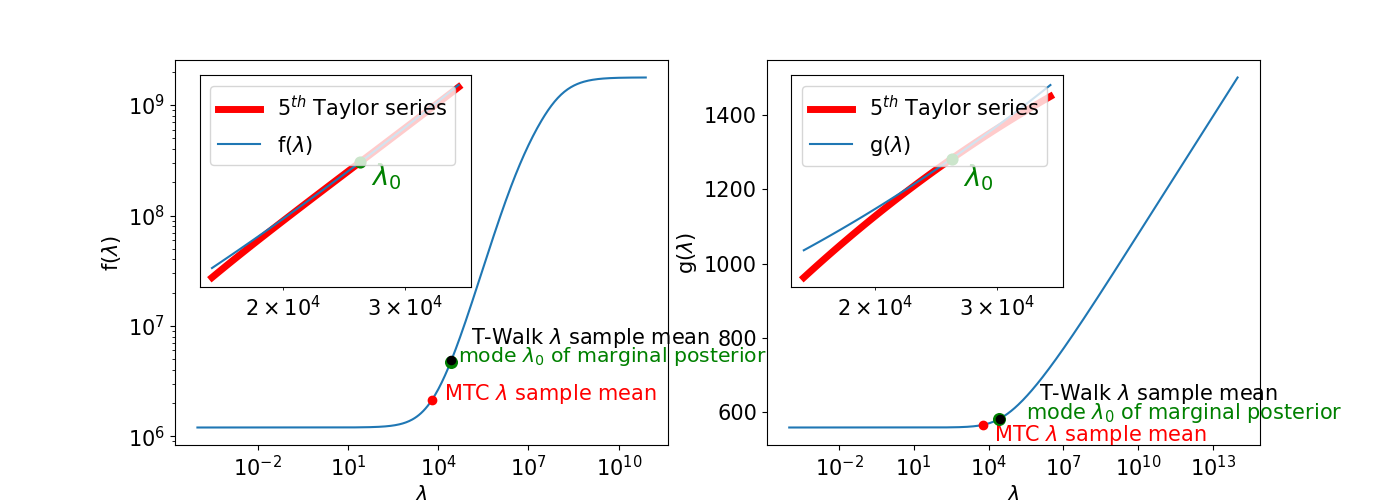
\includegraphics[width=1\textwidth]{f_and_g.png} 
\caption[Plotting $f(\lambda)$ and $g(\lambda)$ for a large range of $\lambda$ to characterize the marginal posterior distribution.]{\textbf{Plotting $f(\lambda)$, Eq. \ref{eq:gtay}, and $g(\lambda)$, Eq.m \ref{eq:gtay}, for a large range of $\lambda$ to characterize the marginal posterior distribution.}
We included the samples mean of the MTC-Sampling (red) and T-walk algorithm (black) \cite{}. In the upper left corner of each figure, we plotted the Taylor series (red) of $f(\lambda)$ and $g(\lambda)$ around the mode of the marginal posterior $\pi(\delta_0, \gamma_0 | \bm{y})$, where $\lambda_0 = \delta_0 / \gamma_0 $. To display the Taylor series we computed up to the fifth derivatives of each function. Note that we usually only focus on a small range of $\lambda$ compared to the here shown range.}
\label{fig:fandg}
\end{figure}
In doing so we set up a specific forward model, in which we specify the number of layers and the number of measurements, to determine the Equations \ref{eq:gammaPrior} and \ref{eq:lamPrior}.
We measure $m = 105$ times equally spaced in between the tangent heights of $2$km and $100$km.
We were given data of $n = 47$ Ozone layers so that the Ozone concentration is zero below 5km and above 90km, as indicated in Figure \ref{fig:forModel}.
We stimulated white noise with a standard deviation of 1\% of the maximum value of data and plotted this in golden color in see Figure \ref{fig:RecRes}.
We calculate the function $f(\lambda)$ and $g(\lambda)$ by using the linear solver \textit{gmres} of the \textit{scipy.sparse.linalg} package in \textit{Python}.
We use the solver to compute the matrix multiplication of $\bm{B}^{-1}\bm{L}$ and $\bm{B}^{-1} \bm{F}^T \bm{y}$, where we set the tolerances for convergence to $10^{-7}$ and repeat the process after 25 iterations.
For a large range of $\lambda$ we plotted $f(\lambda)$ and $g(\lambda)$ in Figure \ref{fig:fandg} and include some results of the sampling process such as sample mean of the MTC-Sampler in red and of the T-Walk algorithm in black.
The top left corner of each figure shows the Taylor approximation around the mode of the marginal posterior distribution in red underneath the original function in blue.

\begin{figure}[thb]
	\centering
		\subfigure[caption]{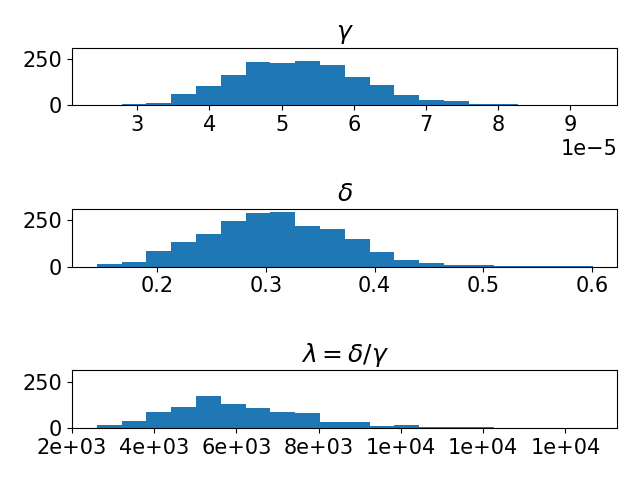
\includegraphics[width=\textwidth]{HistoResults.png}}
 		\subfigure[caption]{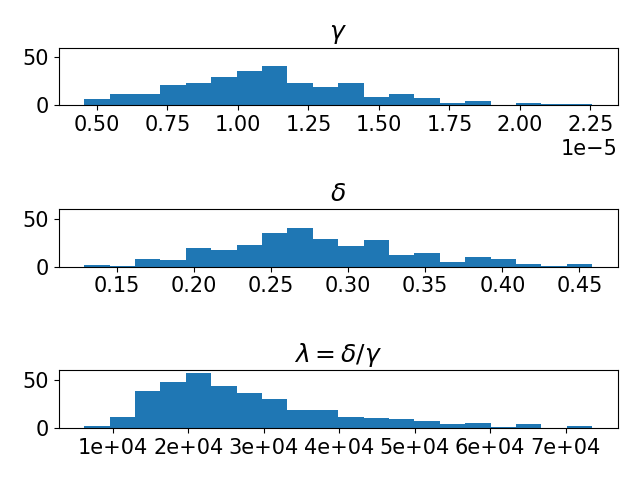
\includegraphics[width=\textwidth]{PyTWalkHistoResults.png}}
\caption[Sampling Results of the MTC-Sampler and the T-Walk algorithm \ref{fig:TWalkHisto}]{\textbf{Sampling Results of the MTC-Sampler \ref{fig:MTCHisto} and the T-Walk algorithm \ref{fig:TWalkHisto}.} The histograms present independent samples of the marginal posterior distribution according to their integrated Auto-correlation time $\tau_{int}$.
Using the \textit{UWerr.m} function by U. Wolff we calculate integrated auto-correlation times of $\tau_{\text{int}, \text{MTC}, \gamma} = 5.4$, $\tau_{\text{int}, \text{MTC}, \delta} = 4.9$ and $\tau_{\text{int}, \text{MTC}, \lambda}= 10.2$ when utilizing the MTC-Sampler with an acceptance rate of 0.34 \cite{Uwerr}.
Running the T-Walk algorithm we obtain following auto-correlation times: $\tau_{\text{int}, \text{T-walk}, \gamma} = 34.1$, $\tau_{\text{int}, \text{T-walk}, \delta} = 34.5$ and $\tau_{\text{int}, \text{T-walk}, \lambda}= 27.5$, with an acceptance rate of 0.42.}
\label{fig:histRes}
\end{figure}
Next, we found the mode at $(\gamma_0, \delta_0) = (1 \times 10^{-5}, 0.26)$ of the marginal posterior distribution by using the \textit{optimize.fmin} function from the \textit{scipy} package in \textit{Python}.
In Figure \ref{fig:fandg} this mode is indicated in green and is the value where we initialize our Markov chain.
We use a normal proposal distribution so that $\lambda' | \lambda \sim \mathcal{N}(\lambda| w^2_{\lambda})$ and draw $10^4$ samples of the marginal posterior distribution, with a burn in period of 50 samples.
We tune variance of the proposal distribution so that the acceptance ratio is between 0.25 and 0.5, and set $w_{\lambda} = 5\times 10^3$.
After calculating the auto-correlation times with \textit{MATLAB} function \textit{UWerr.m} by Ulli Wolff we calculate integrated auto-correlation times \cite{Uwerr}.
Note that we use two times the values of the output of that function, as indicated in \cite{fox2016fast}.
Given the integrated auto-correlation times, we can generate independent samples of the marginal posterior distribution $\pi(\lambda, \gamma | \bm{y})$, see Figure \ref{fig:histRes}.
The integrated auto-correlation times of the MTC-Sampler are: $\tau_{\text{int}, \text{MTC}, \gamma} = 5.4$, $\tau_{\text{int}, \text{MTC}, \delta} = 4.9$ and $\tau_{\text{int}, \text{MTC}, \lambda}= 10.2$.
This is significantly lower compared to the T-Walk algorithm, which needs more than 34 samples to draw two independent hyper-parameter values.
\mccorrect{We indicated the sample mean in Figure} \ref{fig:fandg}\mccorrect{and would like to point out that the T-walk algorithm hits the precalculated mode of the marginal posterior quite accurately.
The MTC-Sampler seems to have a bigger $\gamma$ sample mean compared to the true value.
This reduces the value of $\lambda$ from around $2 \times 10^5$ to $5 \times 10^4$.}

\begin{figure}[htb]
\centering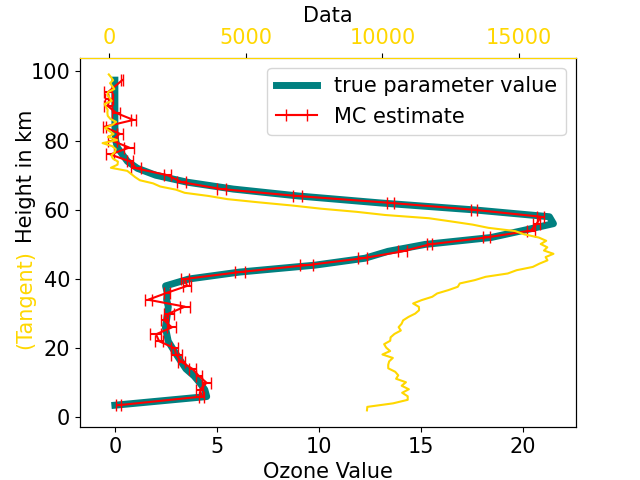
\includegraphics[width=0.7\textwidth]{FirstRecRes.png} 
\caption[Randomize then Optimize (RTO) method to recover the Ozone profile in dependency of the height.]{\textbf{Randomize then Optimize (RTO) method to recover the Ozone profile in dependency of the height.} Here we plotted the mean of 10 posterior samples and their variance in red. We draw hyper-parameter samples according to the samples seen in Figure \ref{fig:MTCHisto}. In green, we displayed the true Ozone profile $\bm{x}$.
We show the data $\bm{y}$ including noise in golden for each tangent height.}
\label{fig:RecRes}
\end{figure}
Given the samples obtained by the MTC-Sampler, see Figure \ref{fig:MTCHisto}, we draw hyper-parameters from the marginal posterior accordingly.
The Randomize then Optimize (RTO) method allows us to compute parameter samples from the full posterior $\pi(\bm{x},\lambda, \gamma|\bm{y})$.
We solve Equation \ref{eq:RTOapplied} for 10 independent hyper-parameter samples to obtain 10 parameter samples.
We plot the results in Figure \ref{fig:RecRes}, where the red line indicates the sample mean including the sample variance.
The results match up well with the true Ozone profile plotted in green.
We included the data $\bm{y}$ in dependency of the tangent height in golden color.

%######################### ideas #####################

% The main goal of this thesis is to apply the introduced samplers to atmospheric trace gas measurements.
% Here we introduce a atmospheric model first a linear model and then raise complexity for the non-linear case.
% The model is suitable to describe a measurement process for a LIMB-Sounder

% \mccorrect{Maybe at the beginning.. or mention at the beginning that this is the motivation for this work.. speed up sampling.. can we deliver real time data?}

% \begin{itemize}
%     \item figure of atmosphere
%     \item Limb sounder - basic principles
%     \item linear model
%     \item non linear model
% \end{itemize}



% -how to sep up a model
% - scaling of the froward map and scaling
% -hyperparameter
% -sample from hyperpriors


